\section{Multi-armed Bandits}

\subsection*{Exercise 2.1: Two-armed Test Bed}

The probability of choosing the greedy arm is the probability of exploiting plus the probability of randomly choosing the greedy arm when exploring:

\vspace{-6mm}
\begin{align}
P(Greedy) &= P(Exploit) + P(Greedy | Explore) \nonumber \\
 &= 1 - \epsilon + \frac{\epsilon}{numArms} \label{eqn:2_pgreedy} \\
 &= 0.5 + \frac{0.5}{2} \nonumber \\
 &= 0.75 \nonumber
\end{align}

\subsection*{Exercise 2.2: Bandit Example}

It is impossible to determine if an action was definitely greedy from the information given - the agent could explore but happen to choose the greedy option at random, resulting in an action that appears greedy but was in fact exploratory. It is only viable to say if the action was exploratory or possibly exploratory, however one could argue that it is arbitrary whether the agent took the greedy action or explored and randomly selected the greedy action since the outcome is the same. The clearest way to evaluate which actions were definitely exploratory and which were not is to examine the action-value estimates over time:

\vspace{-6mm}
\begin{center}
\renewcommand{\arraystretch}{1.2}
\begin{tabular}{c|c|c|c|c|c|c|c}
    \textbf{Time} & \textbf{Arm 1} & \textbf{Arm 2} & \textbf{Arm 3} & \textbf{Arm 4} & \textbf{Greedy} & \textbf{Action} & \textbf{Reward} \\ 
	\hline 
	1 & 0 & 0 & 0 & 0 & Any & 1 - Possibly exploratory & 1 \\ 
	\hline 
	2 & 1 & 0 & 0 & 0 & 1 & 2 - Exploratory & 1  \\ 
	\hline 
	3 & 1 & 1 & 0 & 0 & 1 or 2 & 2 - Possibly exploratory & 2 \\ 
	\hline 
	4 & 1 & 1.5 & 0 & 0 & 2 & 2 - Possibly exploratory & 2 \\ 
	\hline 
	5 & 1 & 1.666... & 0 & 0 & 2 & 3 - Exploratory & 0 \\ 
\end{tabular}  
\end{center}

\subsection*{Exercise 2.3: Greedy vs \boldmath$\epsilon$-Greedy}

The $\epsilon$-greedy methods are clearly better than the greedy method, therefore it is only necessary to consider the two $\epsilon$-greedy methods. As the action-values converge, the optimal value selection also converges. When the action-values converge, the behaviour for the agent is given by Equation \ref{eqn:2_pgreedy}, which is the upper bound for the probability of selecting the greedy action. By substituting in the relative values of $\epsilon$ for the two methods, it is found that the $\epsilon=0.1$ method is limited to 91\% optimal action selection and the $\epsilon=0.01$ method is limited to 99.1\% optimal action selection, meaning given infinite time steps the $\epsilon=0.01$ method will have a higher cumulative reward as it will select the optimal action more often. Based on these limits, the improvement in optimality selection of the $\epsilon=0.01$ method over the $\epsilon=0.1$ method will tend towards $\sim1.088$. This limit, along with a clear demonstrate that the $\epsilon=0.01$ method is more optimal than the $\epsilon=0.1$ method, is shown in Figure \ref{fig:ex2.3_opt-comp}.

\begin{figure}[h]
	\centering
	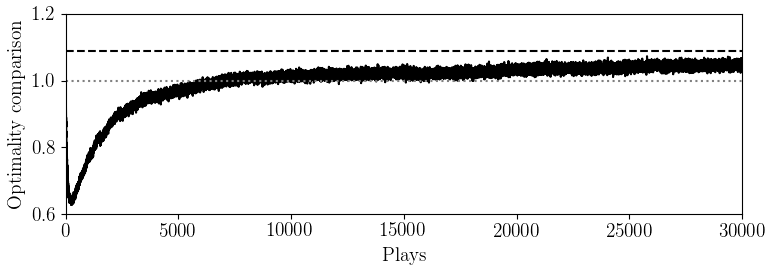
\includegraphics[scale=0.8]{{chapter02/ex2.3_opt-comp}.png}
	\caption{A comparison of the optimality of two $\epsilon$-greedy methods, one with $\epsilon=0.1$ and one with $\epsilon=0.01$. The optimality of the two methods was compared by dividing the percentage optimality selection of the $\epsilon=0.01$ method by the percentage optimality selection of the $\epsilon=0.1$ method. The results were averaged over 2000 random and independently chosen bandit tasks, each run for 30000 plays. It is clear to see that $\epsilon=0.01$ is a better choice in the long run as it results in more optimal selection after $\sim7000$ plays. The dotted line is a guide to show that the optimality comparison goes above one and remains above it. The dashed line indicates the limit that the optimality comparison converges to ($\sim1.088$) as derived above.}
	\label{fig:ex2.3_opt-comp}
\end{figure}


\begin{tcolorbox}
In Section 2.5: Tracking a Non-stationary problem, it is mentioned that a constant step-size results in a weighted average of past rewards, and that the sum of the weights $(1-\alpha)^n + \sum_{i=1}^{n} \alpha(1-\alpha)^{n-1}=1$, which the reader is encouraged to check. Below is a proof of the given statement: 

\vspace{-6mm}
\begin{align*}
S &= (1-\alpha)^n + \sum_{i=1}^{n} \alpha(1-\alpha)^{n-1}  \\
&= (1-\alpha)^n + \alpha(1-\alpha)^{n-1} + \alpha(1-\alpha)^{n-2} + \cdots + \alpha(1-\alpha) + \alpha \\
&= (1-\alpha)(1-\alpha)^{n-1} + \alpha(1-\alpha)^{n-1} + \alpha(1-\alpha)^{n-2} + \cdots + \alpha(1-\alpha) + \alpha \\
&= (1-\alpha)^{n-1}(1-\alpha+\alpha) + \alpha(1-\alpha)^{n-2} + \cdots + \alpha(1-\alpha) + \alpha \\
&= (1-\alpha)^{n-1} + \alpha(1-\alpha)^{n-2} + \cdots + \alpha(1-\alpha) + \alpha \\
& \ \, \vdots \\
&= 1-\alpha+\alpha \\
&=1
\end{align*}

\end{tcolorbox}

\subsection*{Exercise 2.4: Arbitrary Step-size Parameter Weighting}

To determine the weighting of each prior reward for $Q_{n+1}$ when the step-size parameters, $\alpha_{n+1}$, are not constant, a derivation similar to the one for constant step size can be used:

\vspace{-6mm}
\begin{align*}
Q_{n+1} &= Q_n + \alpha_n(R_n - Q_n) \\
&= \alpha_nR_n + (1 - \alpha_n)Q_n \\
&= \alpha_nR_n + (1 - \alpha_n)\alpha_{n-1}R_{n-1} + (1 - \alpha_n)(1-\alpha_{n-1})Q_{n-1} \\
&= \alpha_nR_n \\ 
& \quad + (1 - \alpha_n)\alpha_{n-1}R_{n-1} \\
& \quad + (1 - \alpha_n)(1 - \alpha_{n-1})\alpha_{n-2}R_{n-2} \\
& \quad + (1 - \alpha_n)(1 - \alpha_{n-1})(1 - \alpha_{n-2})\alpha_{n-3}R_{n-3} \\
& \quad \ \, \vdots \\
& \quad + (1 - \alpha_n)(1-\alpha_{n-1}) \cdots (1-\alpha_3)\alpha_2R_2 \\
& \quad + (1 - \alpha_n)(1-\alpha_{n-1}) \cdots (1-\alpha_2)\alpha_1R_1 \\
& \quad + (1 - \alpha_n)(1-\alpha_{n-1}) \cdots (1-\alpha_1)Q_1 \\
&= \alpha_nR_n + \sum_{i=2}^{n}\Big(\alpha_{i-1}R_{i-1}\prod_{j=i}^{n}(1-\alpha_j)\Big) + Q_1\prod_{i=1}^{n}(1-\alpha_i) \numberthis \label{eqn:2_param-weight} \\
\end{align*}

\subsection*{Exercise 2.5: Non-stationary Problems}

To compare constant step-size and sample-average methods on non-stationary bandit problems, both methods were applied to 2000 random and independently chosen non-stationary bandit tasks (as per the other experiments in the text) which ran for 10000 plays. As expected, the constant step-size method performed better than the sample-average technique as it was able to track the optimal arm with greater accuracy; see Figure \ref{fig:ex2.5_non-stat}. 

\begin{figure}[h!]
	\centering
	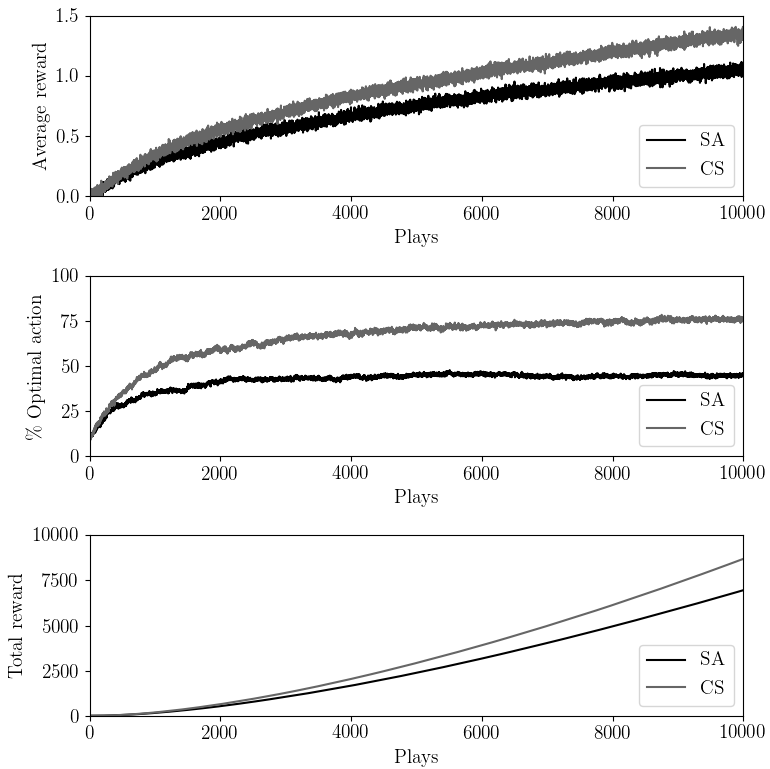
\includegraphics[scale=0.78]{{chapter02/ex2.5_non-stat}.png}
	\caption{A comparison of the constant step-size (CS) method with the sample-average (SA) method on a non-stationary multi-armed bandit problem. It is clear to see that CS outperforms SA, reaching more optimal action selection and thus greater total reward over time.}
	\label{fig:ex2.5_non-stat}
\end{figure}

\subsection*{Exercise 2.6: Mysterious Spikes}

The mysterious spikes seen when using optimistic action selection are dependent on the number of arms used in the bandit scenario. The first spike is the most significant and easiest to explain - the optimistic initial values mean each of the $n$ arms is pulled at least once before any arm is pulled twice, so the $n+1^{th}$ selection will be the first realistic arm choice, and assuming it is a greedy choice, there is a good chance it is the optimal arm as the algorithm has approximate value estimates for each arm already, hence the sudden jump in optimality choice after the first $n$ pulls. However, if the optimal arm is pulled on the $n + 1^{th}$ play, it could produce a poor value due to the noise of the arm values, resulting in an estimate for the optimal arm that is below the other arm estimates, so the optimal arm is not selected for subsequent plays. This leads to the second, smaller spike that occurs on the $2n + 1^{th}$ pull - each arm is tried once more, resulting in more accurate estimates for each arm and thus a more likely optimal choice after $2n$ pulls. This idea was confirmed through reimplementing the results in the text and examining the plays on which the spikes occur; they were indeed on the $n+1^{th}$ and $2n + 1^{th}$ pulls.

\subsection*{Exercise 2.7: Unbiased Constant Step-Size Trick}

To show that the step-size of $\beta_n = \alpha/\bar{o}_n$ produces an exponential recency-weighted average without initial bias, it is sufficient to show that the term for $Q_1$ in Equation \ref{eqn:2_param-weight} disappears when using this step-size. Thus it need only be shown that $\prod_{i=1}^{n}(1-\beta_i) = 0$. The first step in proving this is to find $\bar{o}_{n+1}$ in terms of $\alpha$:

\vspace{-6mm}
\begin{align*}
\bar{o}_{n+1} &= \bar{o}_n + \alpha(1 - \bar{o}_n) \\
&= \alpha + (1-\alpha)\bar{o}_n \\
&= \alpha + (1-\alpha)\alpha + (1-\alpha)^2\bar{o}_{n-1} \\
&= \alpha + (1-\alpha)\alpha + (1-\alpha)^2\alpha + \cdots + (1-\alpha)^t\alpha \\
&= \alpha\sum_{i=0}^{n}(1-\alpha)^i
\end{align*}

This allows $\beta_{n+1}$ to also be found just in terms of $\alpha$:

\vspace{-6mm}
\begin{align*}
\beta_{n+1} &= \frac{\alpha}{\bar{o}_{n+1}} \\
&= \frac{\alpha}{\alpha\sum_{i=0}^{n}(1-\alpha)^i} \\
&= \sum_{i=0}^{n}(1-\alpha)^{-i}
\end{align*}

As a result of the above, $\beta_1 = 1$, which proves $\prod_{i=1}^{n}(1-\beta_i) = 0$, meaning $\beta_n$ does indeed give an exponential recency-weighted average without initial bias.

\subsection*{Exercise 2.8: UCB Spike}

The spike in performance on the $11^{th}$ step when using the UCB algorithm shows a large increase in performance but then a decrease, albeit to a level much greater than before the spike. After the opening ten plays in which each arm is pulled once, the square-root term in the UCB action selection method is equal for all of the arms, therefore the $11^{th}$ pull is selected solely based on the arm estimates found from the first ten pulls, resulting in a greedy choice of arm which is likely to be a good if not optimal arm, hence the immediate increase in performance on the $11^{th}$ play. On the $12^{th}$ play, the square-root term is no longer the same for each arm - for the previously selected arm it is reduced by a factor of $\sqrt{2}$. As a result, other arms could have a greater score as evaluated by the UCB method, despite having potentially worse estimates. This is compounded by the fact than the previously selected arm may have a `bad' pull (return a value below its expected value), resulting in an estimate below the true value. Both of these factors result in the decrease in performance on the $12^{th}$ play as non-optimal arm selection becomes more likely. A larger value for $c$ increases the the effect of the $\sqrt{2}$ factor in the UCB action selection, as more emphasis is placed on the square-root factor rather than the value estimate. 

\subsection*{Exercise 2.9: Two-case Softmax}

The sigmoid function mentioned is of the form $1/(1+e^{-x})$. The equivalence of the two-case softmax distribution with the sigmoid function is shown below, for actions $a_1$ and $a_2$:

\vspace{-6mm}
\begingroup
\addtolength{\jot}{0.5em}
\begin{align*}
\pi_t(a_1) &= \frac{e^{H_t(a_1)}}{\sum_{b=1}^{k}e^{H_t(b)}} \\
&= \frac{e^{H_t(a_1)}}{e^{H_t(a_1)} + e^{H_t(a_2)}} \\
&= \frac{1}{1 + e^{H_t(a_2) - H_t(a_1)}} \\
&= \frac{1}{1 + e^{-x}} & \text{where} \ x = H_t(a_1) - H_t(a_2)
\end{align*}
\endgroup